%
% mental-model-paper.tex
%
% This is the LaTex source file for a paper on the role the alignment of user and developer mental models play in the usability of skeuomorhpic interfaces.
%

%
% Use the standard article template.
%
\documentclass{article}

% The geometry package allows for easy page formatting.
\usepackage{geometry}
\geometry{letterpaper}

% Load up special logo commands.
\usepackage{doc}

% Package for formatting URLs.
\usepackage{url}

% Packages and definitions for graphics files.
\usepackage{graphicx}
\usepackage{epstopdf}
\DeclareGraphicsRule{.tif}{png}{.png}{`convert #1 `dirname #1`/`basename #1 .tif`.png}

%
% Set the title, author, and date.
%
\title{Skeuomorphism and Mental Models}
\author{Britain Southwick}
\date{October 30, 2012}

%
% The document proper.
%
\begin{document}

% Add the title section.
\maketitle

% Add an abstract.
\abstract{
Skeuomorphic interfaces have experienced a huge surge in popularity in recent years. This can be attributed, in part, to the ease with which they allow the developer to align their mental model of the software or app with that of the consumer. When done right and in the right context, skeuomorphic interfaces present an easy to use, flavorful, and inviting atmosphere that makes the software much more popular among consumers. However, there are certainly cases where a skeuomorphic interface can only serve to confuse and annoy, such as when it is implemented incorrectly or in the wrong type of software. 
}

% Add various lists on new pages.
\pagebreak
\tableofcontents

\pagebreak
\listoffigures

\pagebreak
\listoftables

% Start the paper on a new page.
\pagebreak

%
% Body text.
%
\section{Introduction}
\label{introduction}

	A skeuomorphic interface is described by medialoot.com as "A derivative object that retains ornamental design cues to a structure that was necessary in the original, even when not functionally necessary" \cite{media loot}. In very general terms, a skeuomorphic interface is when an app that simulates a real world object is aesthetically designed to look like whatever it is simulating. Frequently, these designs have no function other than aesthetics. Apple Computers in particular is very fond of using skeuomorphic interfaces. 

	Examples can be found all across their IOS, including the iCalendar, the Calculator, and the Notes app. Skeuomorphic interfaces are generally used for fun, creative apps and software such as painting programs or music creators. Their purpose is to make the app or software seem familiar and interesting to the consumer. With the proliferation of touch based user interfaces like the iPod and the iPad, skeuomorphic interfaces are becoming more and more widespread. The consumer response seems to be generally favorable (indicating why Apple pursues the design so judiciously), but among designers the response is much more divided. Some designers voice vehement opposition while others defend the virtues of skeuomorphism. This paper aims to examine these positions to come to a conclusion as to how effectively skeuomorphism aligns the mental models of the developers and the users.


\section{Background, Preliminary, and Related Work}

	A search for scholarly articles regarding the topic of skeuomorphic user interfaces did not yield any results, but this topic is widely discussed in various blog posts from a variety of user interface designers. Therefore, this paper will use the opinions and knowledge presented by these designers to draw conclusions. I will compare and contrast the different positions of these posts in order to synthesize a conclusion as to whether or not skeuomorphic interfaces ultimately align the mental models of users and developers.

\section{Pros and Cons of Skeuomorphism}
	In this section I will present the benefits and drawbacks of skeuomorphic interfaces as identified by the various blog posts. Lastly, the benefits and drawbacks will be compared and analyzed to reach a conclusion. 

\subsection{Benefits of Skeuomorphism}

	One of the most frequently mentioned benefits of skeuomorphism is that the way skeuomorphs mimic familiar objects leads to increased learnability. Tobias Ahlin, a designer for Spotify, uses the example of iBooks to illustrate how familiarity leads to skeuomorphic apps excelling in the learnability metric. He says "Apple makes it obvious by using a book metaphor that you should swipe your finger over the pages to flick to the next page" \cite{story}. When skeuomorphic design is implemented in apps simulating objects that the majority of users are familiar with, it should take almost no time to learn how to use the app. It is this facet of skeuomorphic interface design that truly aligns the mental models of users and developers. The developers have designed an app that is supposed to simulate reading a book. By making the interface look and behave just like a real book would, users can pick up the app and instantly know how to use it due to their familiarity with real books. The users see exactly what the developers envisioned. Medialoot.com echoes these feeling by using the analogy of flight controls. They say "Users like the feeling of familiarity when they see a new interface. Imagine sitting in the cockpit of a plane for the first time, and trying to fly it. You probably wouldn't have much luck, but trained pilots can fly different types of plane because they are familiar with the controls" \cite{media loot}. Users are able to transfer their knowledge of using existing objects to brand new technology simply because the new apps look and feel familiar to them. This drastically cuts down on the time needed to learn how to use an app, a major limiting factor in how likely the average consumer is to use a product. Software with a very high learning curve, such as the LaTex software I am using right now, tends to only be used by people who absolutely need it or have the patience to learn a new skill to use it. This is perfectly fine for specialty software, but certain apps, like a calendar or a book, need to be useable and appealing to everyone.
	
	Another proposed benefit of skeuomorphic interfaces is that they help the user get in the right frame of mind to use the app. Tobias Ahlin calls this property storytelling. He says "The UI tells a story and sets a mood for the entire experience" \cite{story}. He uses the example of the app Papers, which emulates a notepad in both function and design.  The purpose of the app is to provide the user with a tool to write down ideas and thoughts, but not for serious work. Ahlin notes "The UI not only communicates that [the idea that Papers is not for serious work], but it helps you put yourself in a state where you feel free to express ideas without evaluating them" \cite{story}. To contrast Papers, Ahlin uses the app Brushes to illustrate an app with a very similar function, but a purpose that is completely different. He says that the framing and design of the app would inspire him to commit several hours to the project, not just jot down notes. He concludes "The functionality of Paper and Brushes are basically the same, yet the perceived purpose is totally different" \cite{story}.
	
	Lastly, in a bit of an overlap with the above mentioned benefits, is that skeuomorphic interfaces are able to convey purpose to a variety of different users. To demonstrate this function, Ahlin compares the older version of Apple's PhotoBooth app with the newer version. The older version had a sparse, minimalistic design that was completely functional, but led to some confusion (especially among older generations) as to the purpose of the app. The new version introduced a new interface for the fullscreen view that resembled a traditional photo booth, complete with curtains and wood paneling. Ahlin says "The first version of Photo Booth made all this really easy and accessible. It did not, however, communicate the purpose of Photo Booth: fool around and have fun...In the new fullscreen mode, Apple uses skeuomorphism to invite users to play"\cite{story}. In this case, the introduction of a skeuomorphic interface drastically increased the alignment of the user's mental model with that of the developers.

\subsection{Flaws of Skeuomorphism}

	Not all developers agree with the above mentioned benefits. Quite a few designers have blogged about the inherent flaws of skeuomorphic interfaces. One of the noted flaws is that in certain cases a skeuomorphic interface can obfuscate the purpose of the app and confuse the user. Fred Beecher cites Apple's Calendar and Contacts apps as examples. He states " While they retain the visual form of books, they do not allow you to turn pages by swiping. What's worse, they often respond to swipes by scrolling a list on what appears to be a page, severely conflicting with the user's mental model of a book" \cite{guidelines}. In these cases, functions that have been implemented countless times without skeuomorphic interfaces have been made complicated and confusing by the presence of skueomorphic elements. Users have been able to use digital calendars and contact lists perfectly well in the form of simple tables and lists that convey the developers mental model very well. But here, the mental model of the users is that of a book, but the developers had something else in mind, creating a conflict in mental models.
	It has also been noted that for apps intended purely for productivity, skeuomorphic interfaces can severely impact efficiency, while barely increasing learnability. John Pavlus, of fastcodesign.com, says "And designers have been griping about the skeuomorphic idiocy of desktop calculator apps for ages -- why must we stab at clunky virtual "buttons" with our mouse when an entirely computer-native interface is much more powerful?" \cite{codesign}. The time it takes to navigate the buttons on the calculator is much longer than the time it takes to simply use a keyboard, severely hampering efficiency. The same applies to virtual keyboards that mimic real keyboards. While nice looking, these interfaces, in addition to being irritating and clunky, the skeuomorphism contributes nothing to the app. 

\subsection{Figures}

\begin{figure}
\centering
\includegraphics[width=5in]{iBooks.jpg} 

\caption{Apple's iBooks app demonstrates the familiarity of a well implemented skeuomorphic design}
\label{ibooks}
\end{figure}

\begin{figure}
\centering
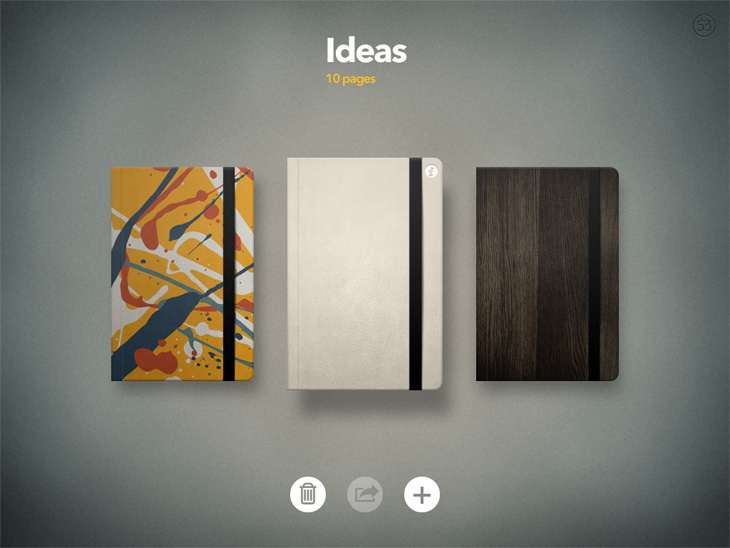
\includegraphics[width=5in]{paperSmall.jpg}
\caption{Papers' skeuomorphic interface helps convey the function of the app.}
\label{Papers}
\end{figure}

\begin{figure}
\centering
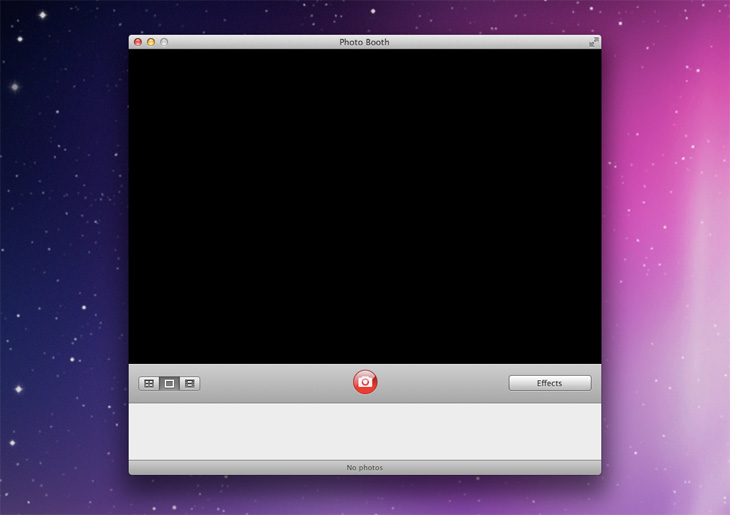
\includegraphics [width=5in]{photoBoothOldSmall.jpg}
\caption{The old version of PhotoBooth left some confusion as to its intended purpose.}
\label{Old Photo Booth}
\end{figure}

\begin{figure}
\centering
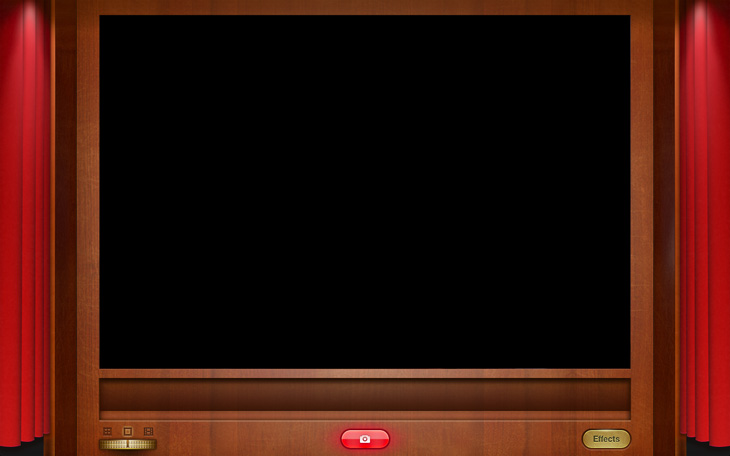
\includegraphics[width=5in]{photoboothFullscreenSmall.jpg}
\caption{The new version makes makes quite clear the purpose the developers had in mind.}
\label{New Photo Booth}
\end{figure}

\begin{figure}
\centering
\includegraphics[width=5in]{contacs.jpg}
\caption{While Apple's Contacts app looks like a book, it hardly behaves like one.}
\label{Contacts}
\end{figure}



\section{Conclusion}

Wrap up your paper with an ``executive summary'' of the paper itself, reiterating its subject and its major points.  If you want examples, just look at the conclusions from the literature.

% Generate the bibliography.
\bibliography{mental-model-paper}
\bibliographystyle{unsrt}

\end{document}
